\section{Architecture}
\label{sec:architecture}

codetopo is organized into four layers: Indexer, Storage, Query Engine, and
MCP Server. Each layer has a single responsibility and communicates with
adjacent layers through a narrow interface.

\begin{figure}[htbp]
\centering
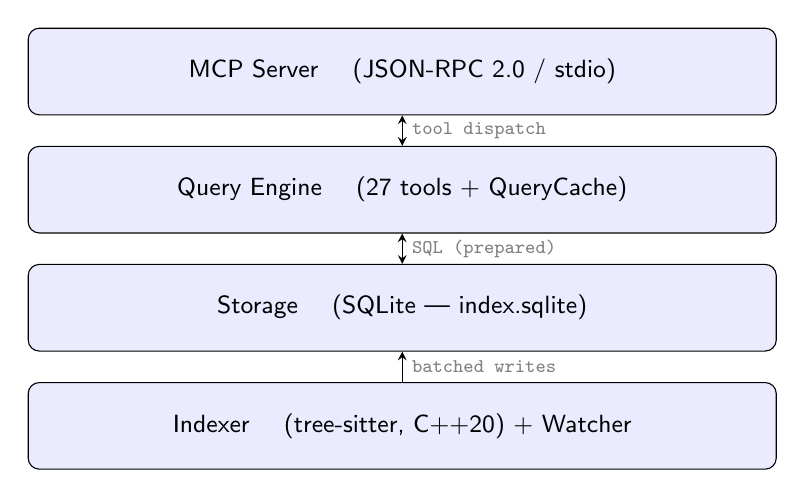
\begin{tikzpicture}[
  layer/.style={draw, fill=blue!8, rounded corners,
                minimum width=9.5cm, minimum height=1.1cm, text centered,
                font=\small\sffamily},
  ann/.style={font=\scriptsize\ttfamily, text=gray},
  >=stealth
]
\node[layer] (mcp)     at (0,4.5) {MCP Server \quad (JSON-RPC 2.0 / stdio)};
\node[layer] (query)   at (0,3.0) {Query Engine \quad (27 tools + QueryCache)};
\node[layer] (storage) at (0,1.5) {Storage \quad (SQLite --- index.sqlite)};
\node[layer] (indexer) at (0,0.0) {Indexer \quad (tree-sitter, C++20) + Watcher};

\draw[<->] (mcp)     -- (query)   node[ann,right,midway] {tool dispatch};
\draw[<->] (query)   -- (storage) node[ann,right,midway] {SQL (prepared)};
\draw[->]  (indexer) -- (storage) node[ann,right,midway] {batched writes};
\end{tikzpicture}
\caption{codetopo four-layer architecture.}
\label{fig:architecture}
\end{figure}

\subsection{Indexer}

The Indexer scans workspace roots, parses each source file with a tree-sitter
grammar~\cite{brunsfeld2018treesitter} appropriate for its language, and
extracts symbols and edges. It writes to the Storage layer in batches within a
single SQLite transaction per file. The Indexer runs at startup (governed by a
\emph{freshness policy}: \texttt{eager}, \texttt{normal}, \texttt{lazy}, or
\texttt{off}) and on demand via the \texttt{reindex} tool.

A platform-native filesystem \emph{watcher} (FSEvents on macOS,
inotify on Linux, ReadDirectoryChangesW on Windows) monitors each workspace
root. On a create, modify, or delete event the watcher schedules an incremental
re-index of the affected file. A branch-switch event (detected by watching
\texttt{.git/HEAD}) triggers re-indexing of all files whose content has changed
since the previous HEAD.

\subsection{Storage}

Storage is a single SQLite database file (\texttt{.codetopo/index.sqlite})
co-located with or near the server binary. It holds the symbol graph, file
metadata, workspace roots, and FTS indexes. The schema is described in detail
in \S\ref{sec:data-model}. SQLite WAL mode allows the Query Engine to serve
reads while the Indexer is writing.

\subsection{Query Engine}

The Query Engine exposes 27 MCP tools. Each tool translates a structured
request into one or more SQL queries, formats the result, and returns it as a
JSON-RPC response. Frequently used statements are cached as \emph{prepared
statements} in a \texttt{QueryCache} keyed by tool name; the cache is
invalidated on each re-index. The tools are organized by capability and
described in \S\ref{sec:mcp-protocol}.

\subsection{MCP Server}

The MCP Server owns the JSON-RPC transport layer (stdio). It performs
protocol negotiation (handshake returns \texttt{protocolVersion 2024-11-05}),
tool registration, and request routing to the Query Engine. Staleness
detection is managed by a \texttt{StalenessState} object that tracks the
mtime of \texttt{.git/HEAD}, the indexed branch/commit, and a
\texttt{\_meta.stale} flag that is included in tool responses when the index
may be out of date.

\subsection{Data flow}

At startup the server opens the database, validates the schema (running
migrations if needed), loads workspace roots, and starts the Indexer for any
root with stale or missing index data (subject to the freshness policy). Once
indexing is complete the server enters its serve loop: it reads JSON-RPC
requests from stdin, dispatches each to the appropriate Query Engine tool via
the prepared-statement cache, and writes the response to stdout.
